\definecolor{dkgreen}{rgb}{0,0.6,0}
\definecolor{gray}{rgb}{0.5,0.5,0.5}
\definecolor{mauve}{rgb}{0.58,0,0.82}

\lstset{frame=none,
  language=Python,
  aboveskip=5mm,
  belowskip=5mm,
  showstringspaces=false,
  columns=flexible,
  basicstyle={\linespread{0.8}\small\ttfamily},
  numbers=none,
  numberstyle=\tiny\color{gray},
  keywordstyle=\color{dkgreen},
  commentstyle=\color{blue},
  stringstyle=\color{mauve},
  breaklines=false,
  breakatwhitespace=true,
  tabsize=3
}

\chapter{Evaluation}

\section{Test and Development Environment}

Millipyde was tested using a desktop workstation with the following specifications: 
\begin{itemize}
  \item Intel Xeon CPU E5-1620 @ 3.50GHz
  \item 32 GB memory
  \item Ubuntu 20.04.3 LTS Operating System
\end{itemize}

The workstation was equipped with two of the following GPU:
\begin{itemize}
  \item AMD Vega 10 XTX (gfx900) GPU
  \item Wavefront size: 64
  \item 64 CUs with 4 SIMDs per CU
  \item 4 Shader Engines
  \item 16KB L1 cache, 4096KB L2 cache
\end{itemize}

\quad Using the system BIOS, the workstation was configured to use large-BAR configuration to expose GPU local memory via PCIe memory BARs. This increased the BAR size to 64 bits, and was required to allow Millipyde to use DMA peer-to-peer memory transfers for any experiments that used both GPUs \cite{rocmrdma}. 

\section{Single Function Benchmarks}

To test performance with individual functions, we used select Millipyde functions that had functionally-equivalent implementations in the non-GPU accelerated library scikit-image. These functions were run on identical images, and their performance was measured using Python's \verb|time.perf_counter| function. This measurement only included the time for the function itself to execute. It excludes the time for the image to be opened and saved. To ensure accuracy and consistency across both implementations, very pixel value in both the scikit-image output and the Millipyde output were compared to 4 decimal places. These benchmark were run on 12 copies of the same image in different sizes. They start at 500 pixels wide and go up to 6000 pixels wide, stepping by 500 pixels every time. 

\subsection{Gamma Correction}

One of the most basic categories of parallel computations are element-wise calculations where each data value in an array undergoes a standalone operation to compute the respective output data value in the resulting array. One such example is Millipyde's \verb|adjust_gamma| function. Each pixel is transformed using the equation $V_{out} = A * V_{in} ^ \gamma$ where  $A$ is a constant multiplier called `gain', and $\gamma$ is the gamma adjustment value. This results in a brightness correction where gamma values less than one increase the overall brightness, and values greater than one decrease the brightness. The effects of this can be seen in Figure \ref{gammaExample}. For our experiments, we ran both the Millipyde function and the scikit-image equivalent with a gamma of 2 and gain of 1.

\begin{figure}[H]
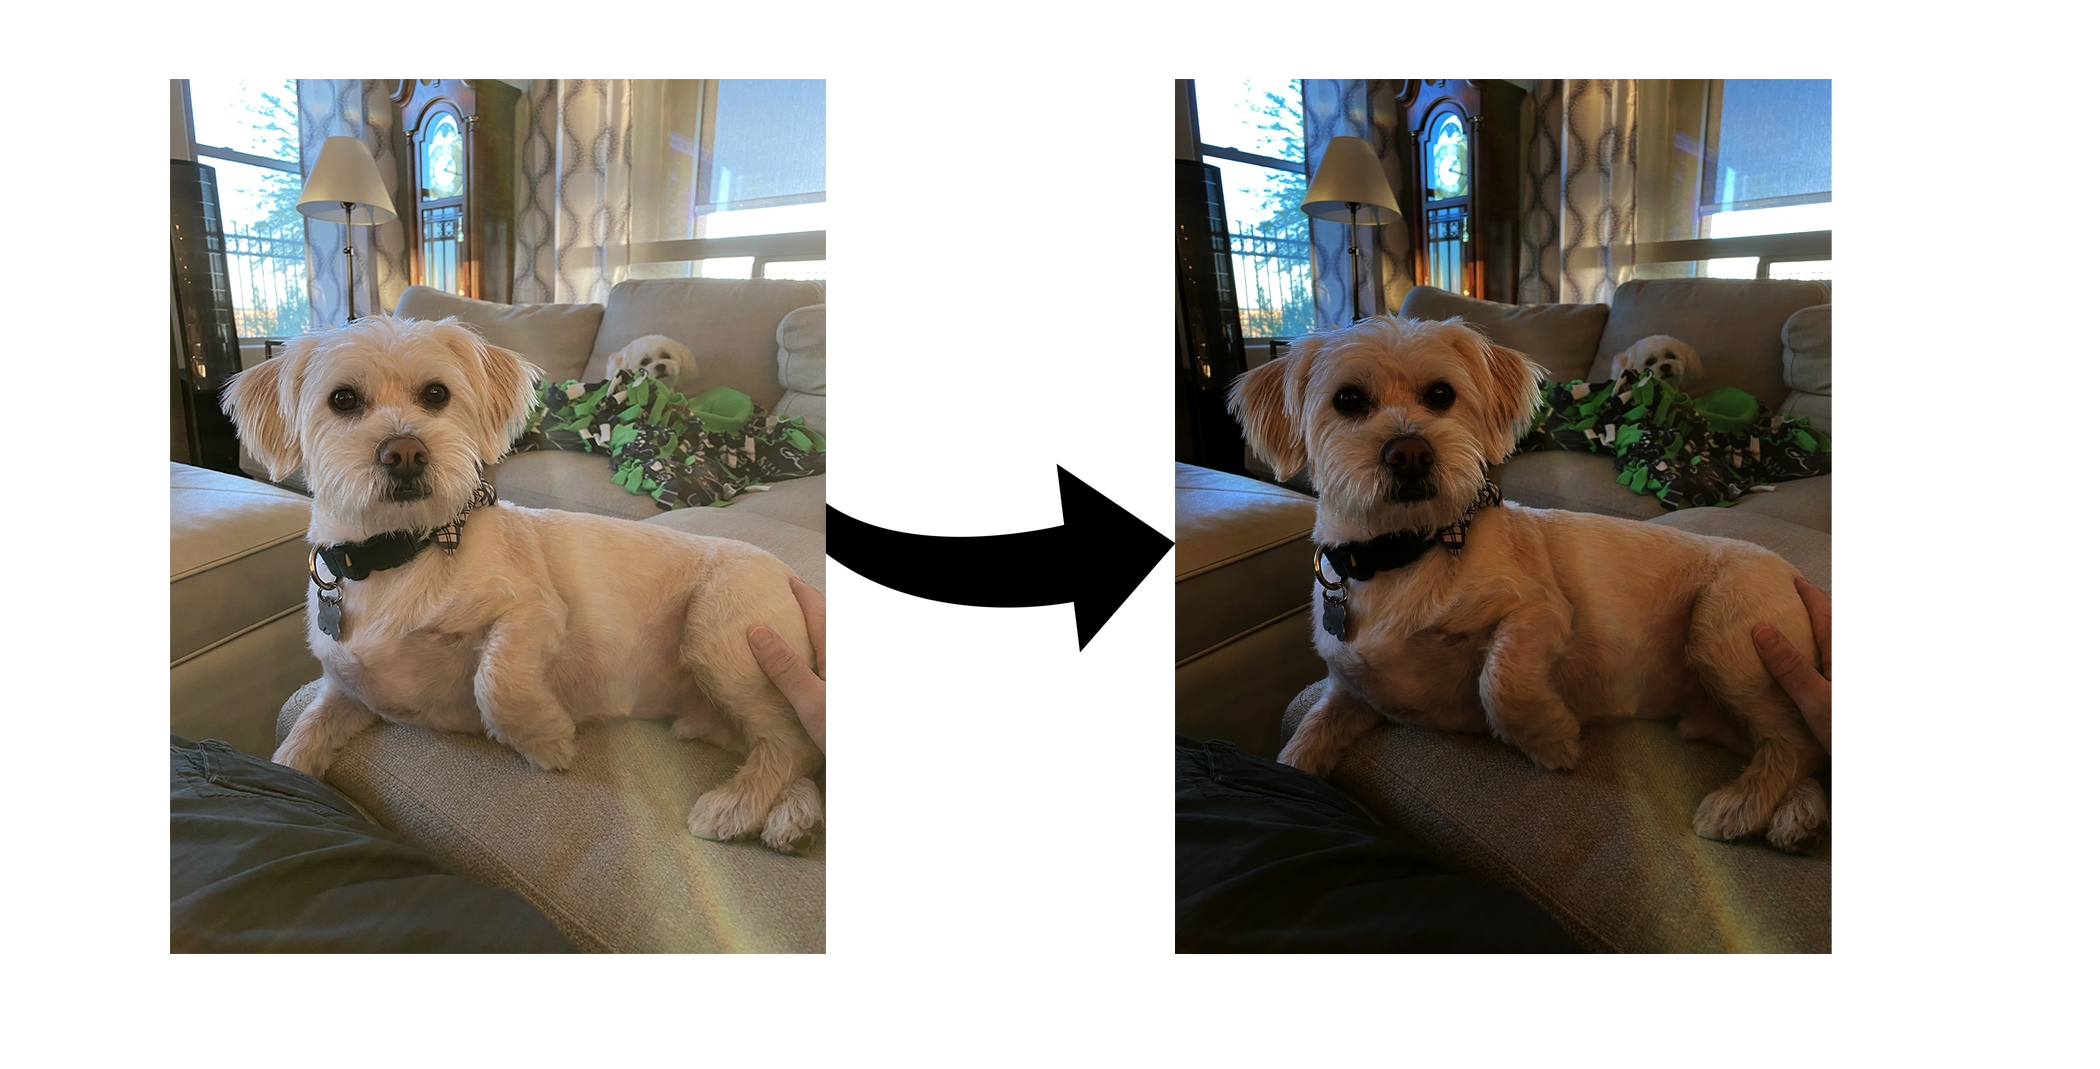
\includegraphics[width=\textwidth]{figures/GammaExample.png}
\centering
\caption{The effects of gamma correction using a gamma value of 2.}
\label{gammaExample}
\end{figure}

\begin{table}[h!]
\centering
\begin{tabular}{ |c|c|c|c| } 
\hline
image size & scikit-image time (s) & Millipyde time (s) & \% difference \\
\hline
500&0.0030651&0.0001561&1964 \\
1000&0.0105069&0.0001869&5622 \\
1500&0.0262136&0.0002929&8950 \\
2000&0.0403756&0.0004912&8220 \\ 
2500&0.0624683&0.0006293&9927 \\
3000&0.0890932&0.0009215&9668 \\
3500&0.1531737&0.0011845&12932 \\
4000&0.1878477&0.0015242&12324 \\
4500&0.2309318&0.0018687&12358 \\ 
5000&0.2741731&0.0022279&12306 \\
5500&0.3252361&0.0027007&12043 \\
6000&0.3819223&0.0031833&11998 \\
\hline
\end{tabular}
\caption{Timing results for gamma correction using scikit-image and Millipyde.}
\label{gammaTable}
\end{table}

\begin{figure}[H]
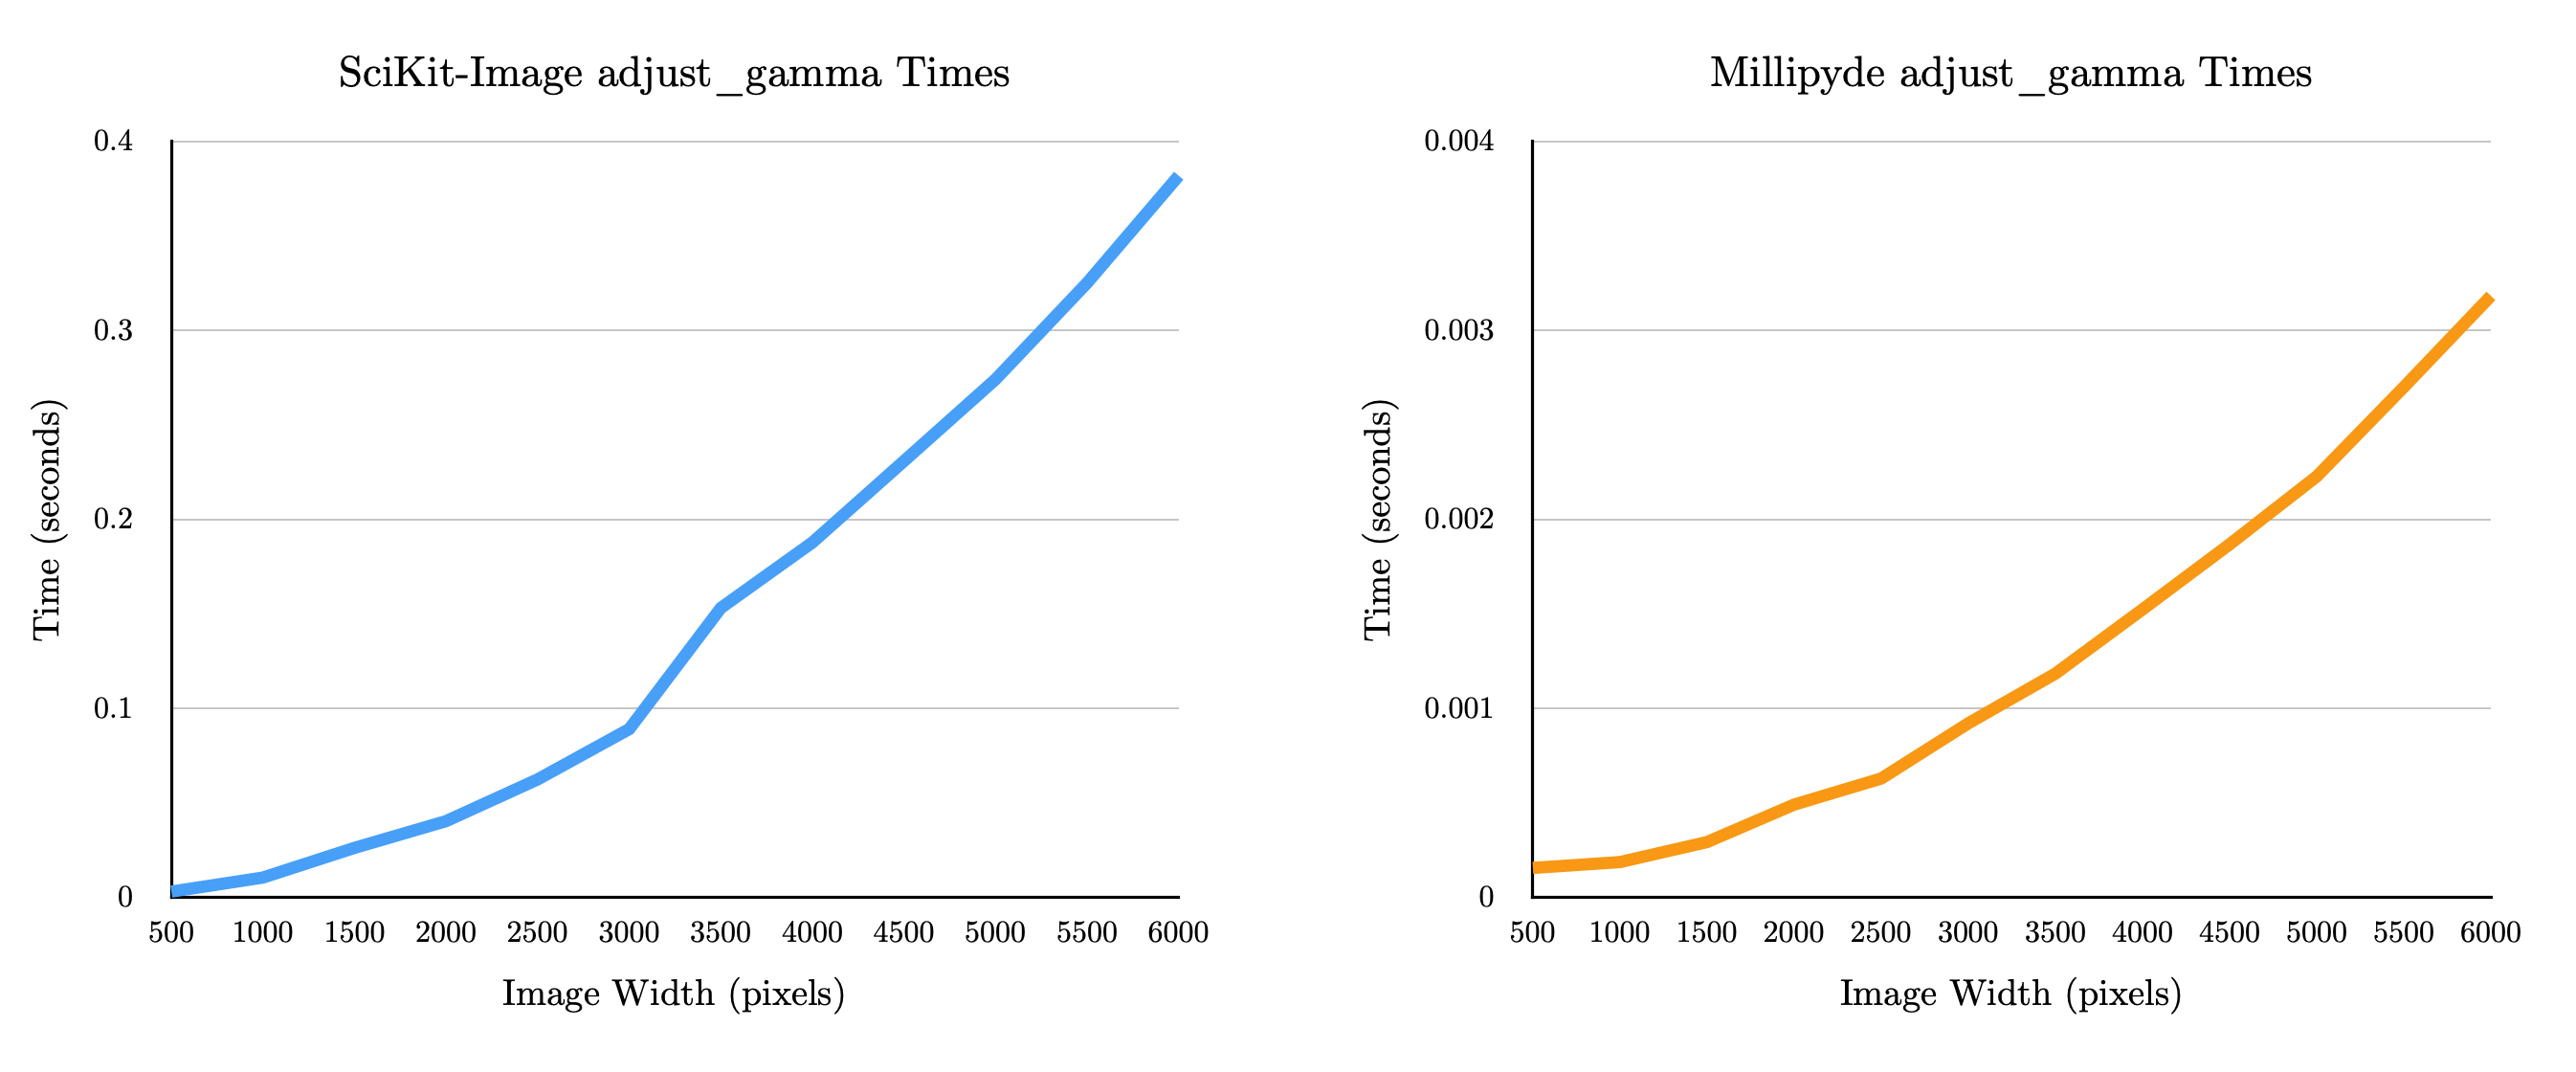
\includegraphics[width=\textwidth]{figures/GammaComparison.png}
\centering
\caption{Graphical representation of the time spent performing gamma correction on an image in scikit-image compared to its GPU-accelerated equivalent in Millipyde.}
\label{gammaComparison}
\end{figure}

\quad The results demonstrated a predictable decrease in runtime for the GPU-accelerated function. It ranged from around 20x faster for the 500-pixel image to more than 100x faster for larger images. These results when graphed followed a clean curve that closely mirrored the scikit-image equivalent as shown in Table \ref{gammaTable} and Figure \ref{gammaComparison}. Users can reliably expect the Millipyde gamma correction functionality to be faster than CPU-only equivalent functions.

\subsection{Greyscale}

 A slightly more complicated variation on a element-wise kernels happens when the dimensions of the input array are different than that of the output array. This can be seen in greyscale conversion functions which translates from a 3-dimensional RGB array of 8-bit integer values to a 2-dimensional array of floating point values. This computation is traditionally done using a weighted sum of the RGB components in an image to produce a single greyscale value between 1 and 0. Both Millipyde and scikit-image use the following weights in this calculation: $Y = 0.2125 R + 0.7154 G + 0.0721 B$ \cite{skirgb2grey}. 
This makes it a good function to use in comparing scikit-image's functionality with the GPU-parallelized implementation in Millipyde. 

\begin{figure}[hbtp]
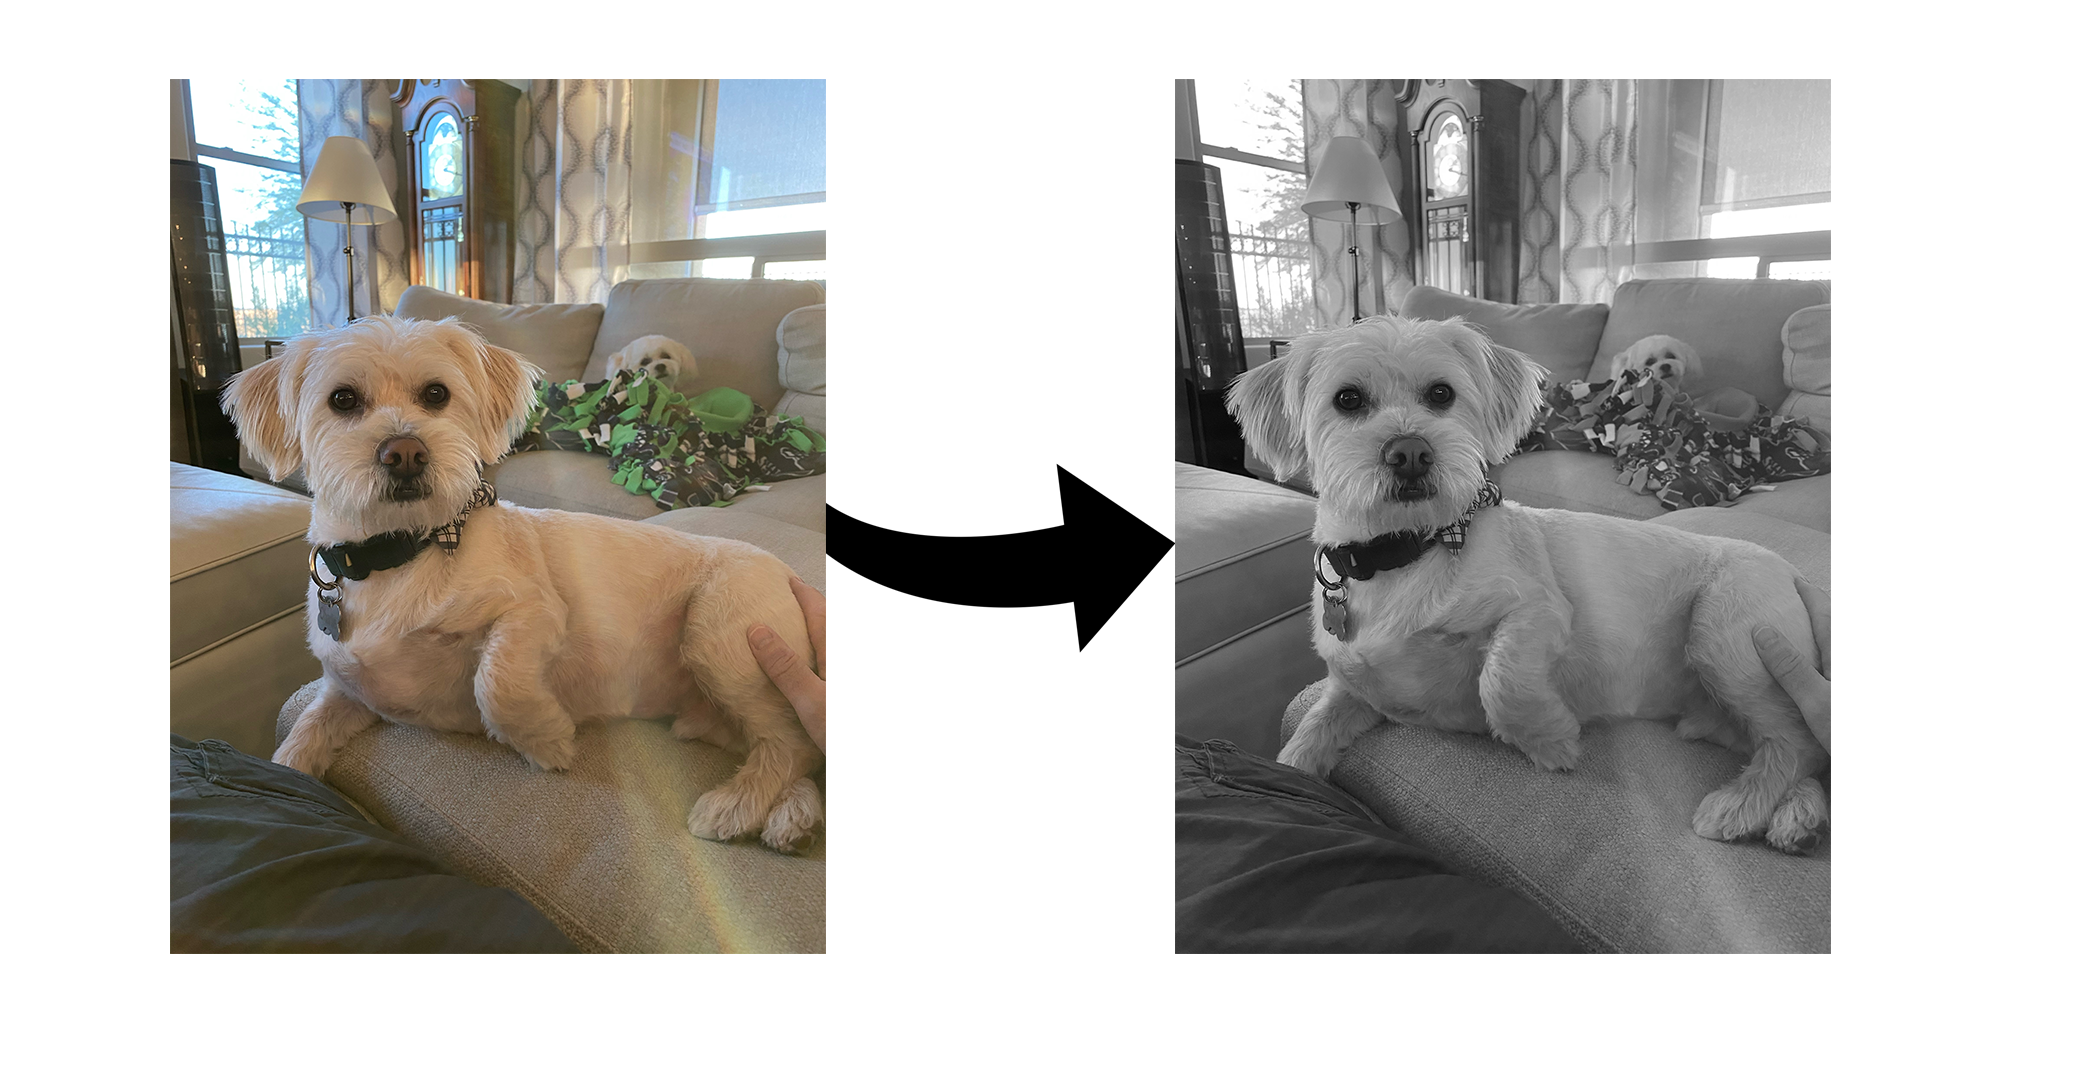
\includegraphics[width=\textwidth]{figures/GreyscaleExample.png}
\centering
\caption{The effects of greyscaling an RGB image.}
\label{greyscaleExample}
\end{figure}

\begin{table}[H]
\centering
\begin{tabular}{ |c|c|c|c| } 
\hline
image size & scikit-image time (s) & Millipyde time (s) & \% difference \\
\hline
500 & 0.0063839 & 0.0014073 & 454 \\
1000 & 0.0260336&0.0014537&1790 \\
1500&0.0535500&0.0052456&1021 \\
2000&0.0942788&0.0055702&1693 \\
2500&0.1466724&0.0054552&2689 \\
3000&0.2102404&0.0065436&3213 \\ 
3500&0.2964064&0.0091423&3242 \\
4000&0.3863234&0.0085288&4530 \\
4500&0.4974762&0.0089737&5544 \\
5000&0.6113694&0.0092912&6580 \\
5500&0.7201406&0.0092047&7824 \\
6000&0.8563366&0.0115259&7516 \\
\hline
\end{tabular}
\caption{Timing results for greyscaling images using scikit-image and Millipyde.}
\label{greyscaleTable}
\end{table}

\begin{figure}[H]
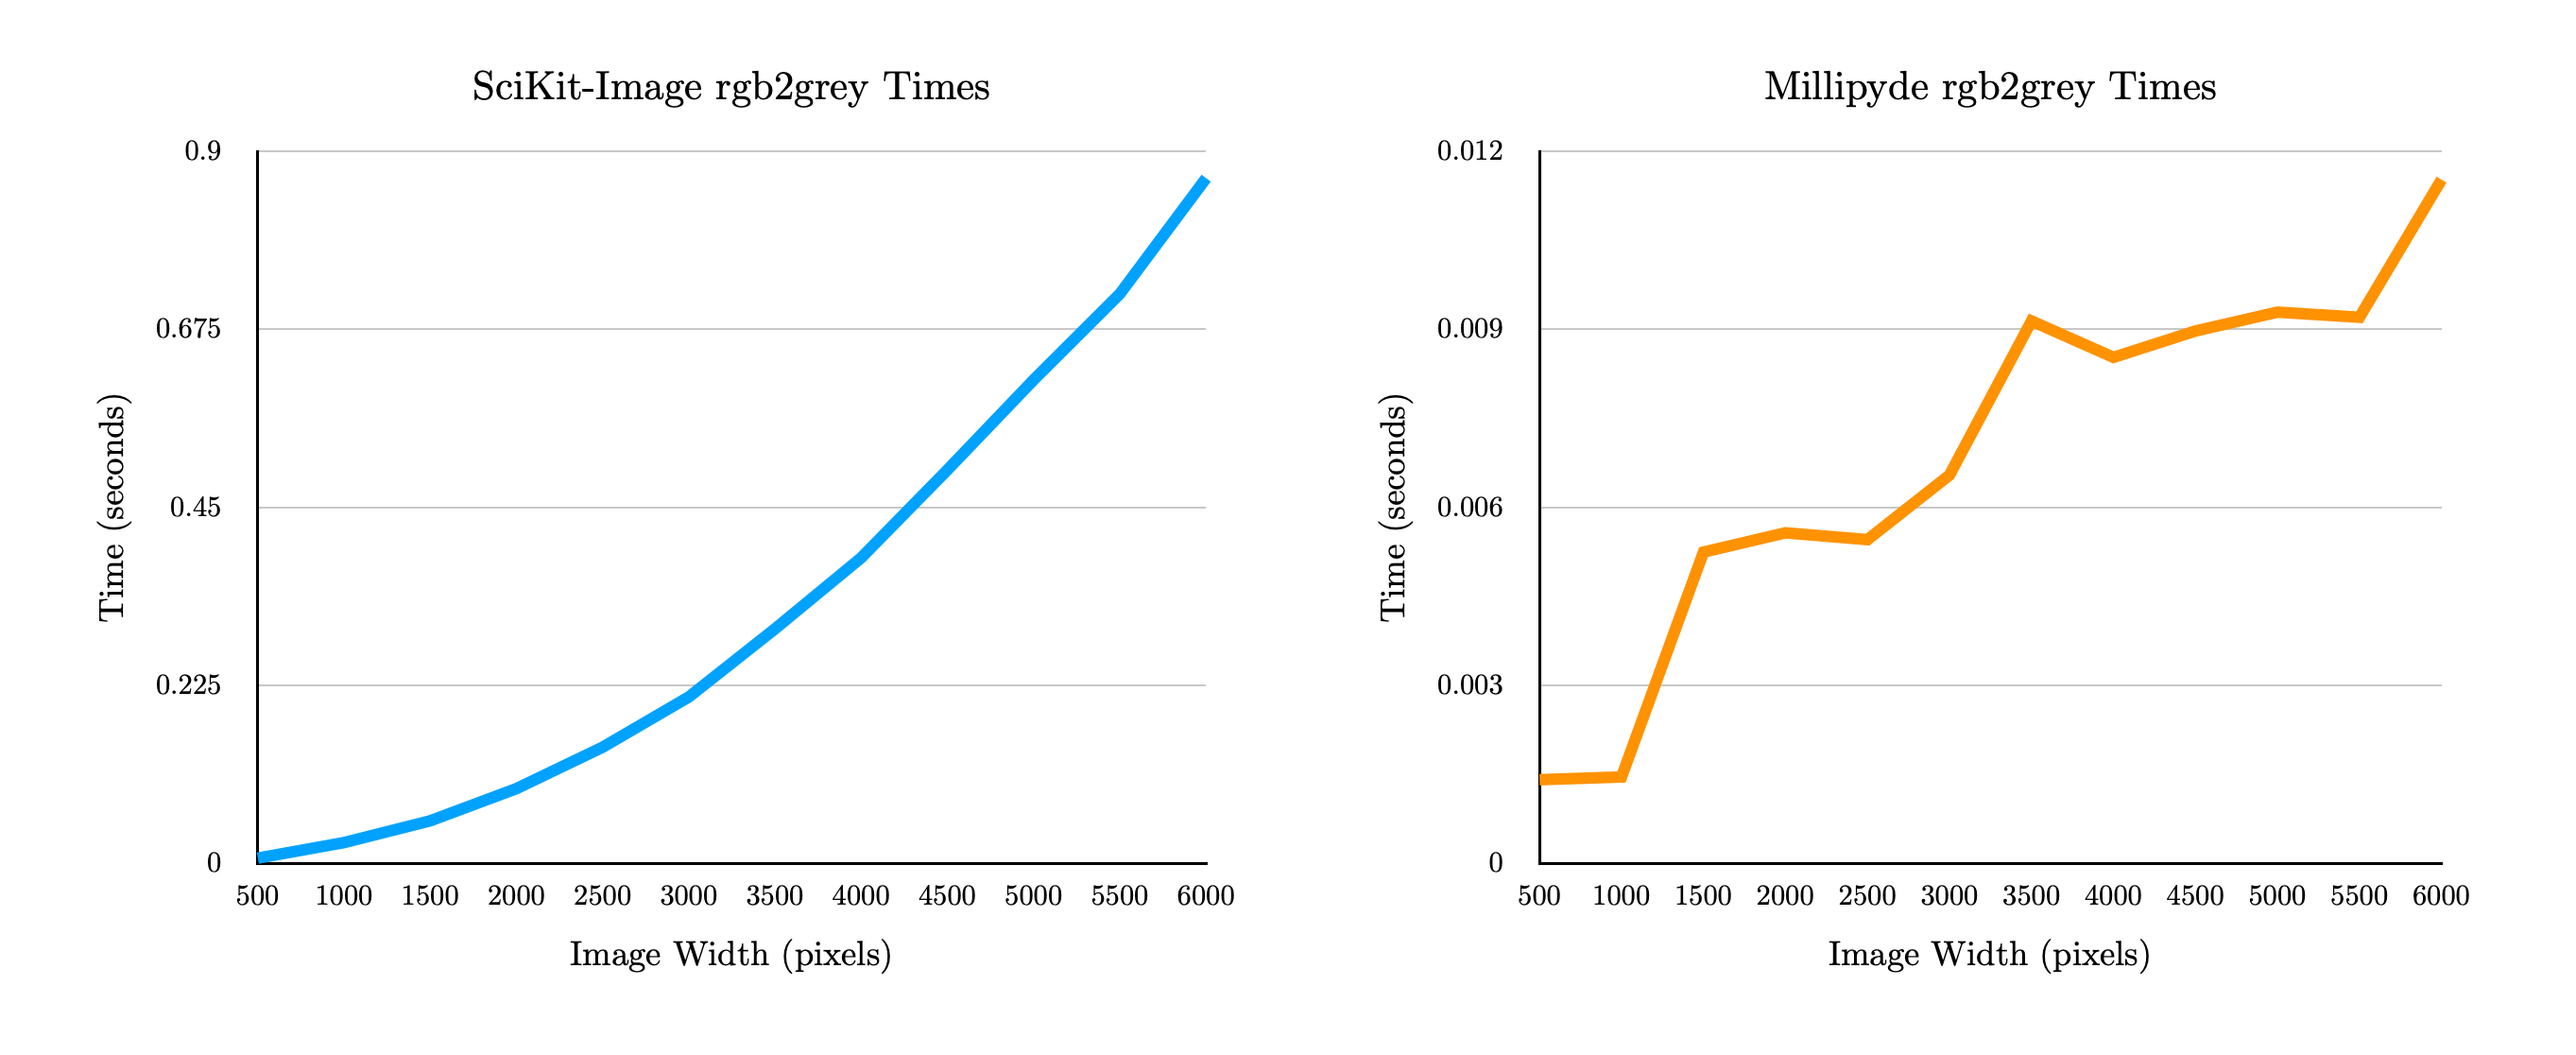
\includegraphics[width=\textwidth]{figures/greyscaleComparison.png}
\centering
\caption{Graphical representation of the time spent greyscaling an image in scikit-image compared to its GPU-accelerated equivalent in Millipyde.}
\label{greyscaleComparison}
\end{figure}

\quad As shown in Table \ref{greyscaleTable} and Figure \ref{greyscaleComparison}, these results differed surprisingly from those of the gamma correction function. On the surface, the kernels for both functions look startlingly similar -- both only perform a single element-wise computation on each input pixel. This difference in performance is therefore likely to do with the difference in shape between the input and output arrays. The resulting Millipyde graph almost resembles stair steps with significant jumps in performance between some image sizes, and stagnated performance between others. We were unable to find a clear cause based on studying the profile results of the function's runtime using the ROCm profiler 'rocprof'. Future experimentation is needed to understand this behavior, and to see if better/more predictable performance is possible. 

\subsection{Gaussian Blur Convolution}

Another large category of parallel computation is the convolution, often referred to as the stencil computation, with applications ranging from signal processing, image processing, video processing, and more \cite{greenBook}. It involves a more mathematically-complex array computation where each output element is a weighted sum of N number of neighboring elements. The weights come from an input mask array called the kernel. For this example, we will use a Gaussian blur convolution which is commonly used in image processing and computer vision for applications such as edge detection \cite{gaussEdge}. For this computation, the kernel can be modeled as a 2D convolution using the kernel $G(x, y) = \frac{1}{2 \pi \sigma^2} e^{-\frac{x^2 + y^2}{2 \sigma^2}}$ where $\sigma$ represents standard deviation. This results in a symmetric kernel with stronger weights in the middle. The Gaussian blur is also separable, meaning the same result can be achieved by a separate pass of a 1-dimensional Gaussian kernel on each axis. The calculation for the 1-dimensional kernel is $G(x) = \frac{1}{\sqrt{2 \pi \sigma^2}} e^{-\frac{x^2}{2 \sigma^2}}$.

\begin{figure}[H]
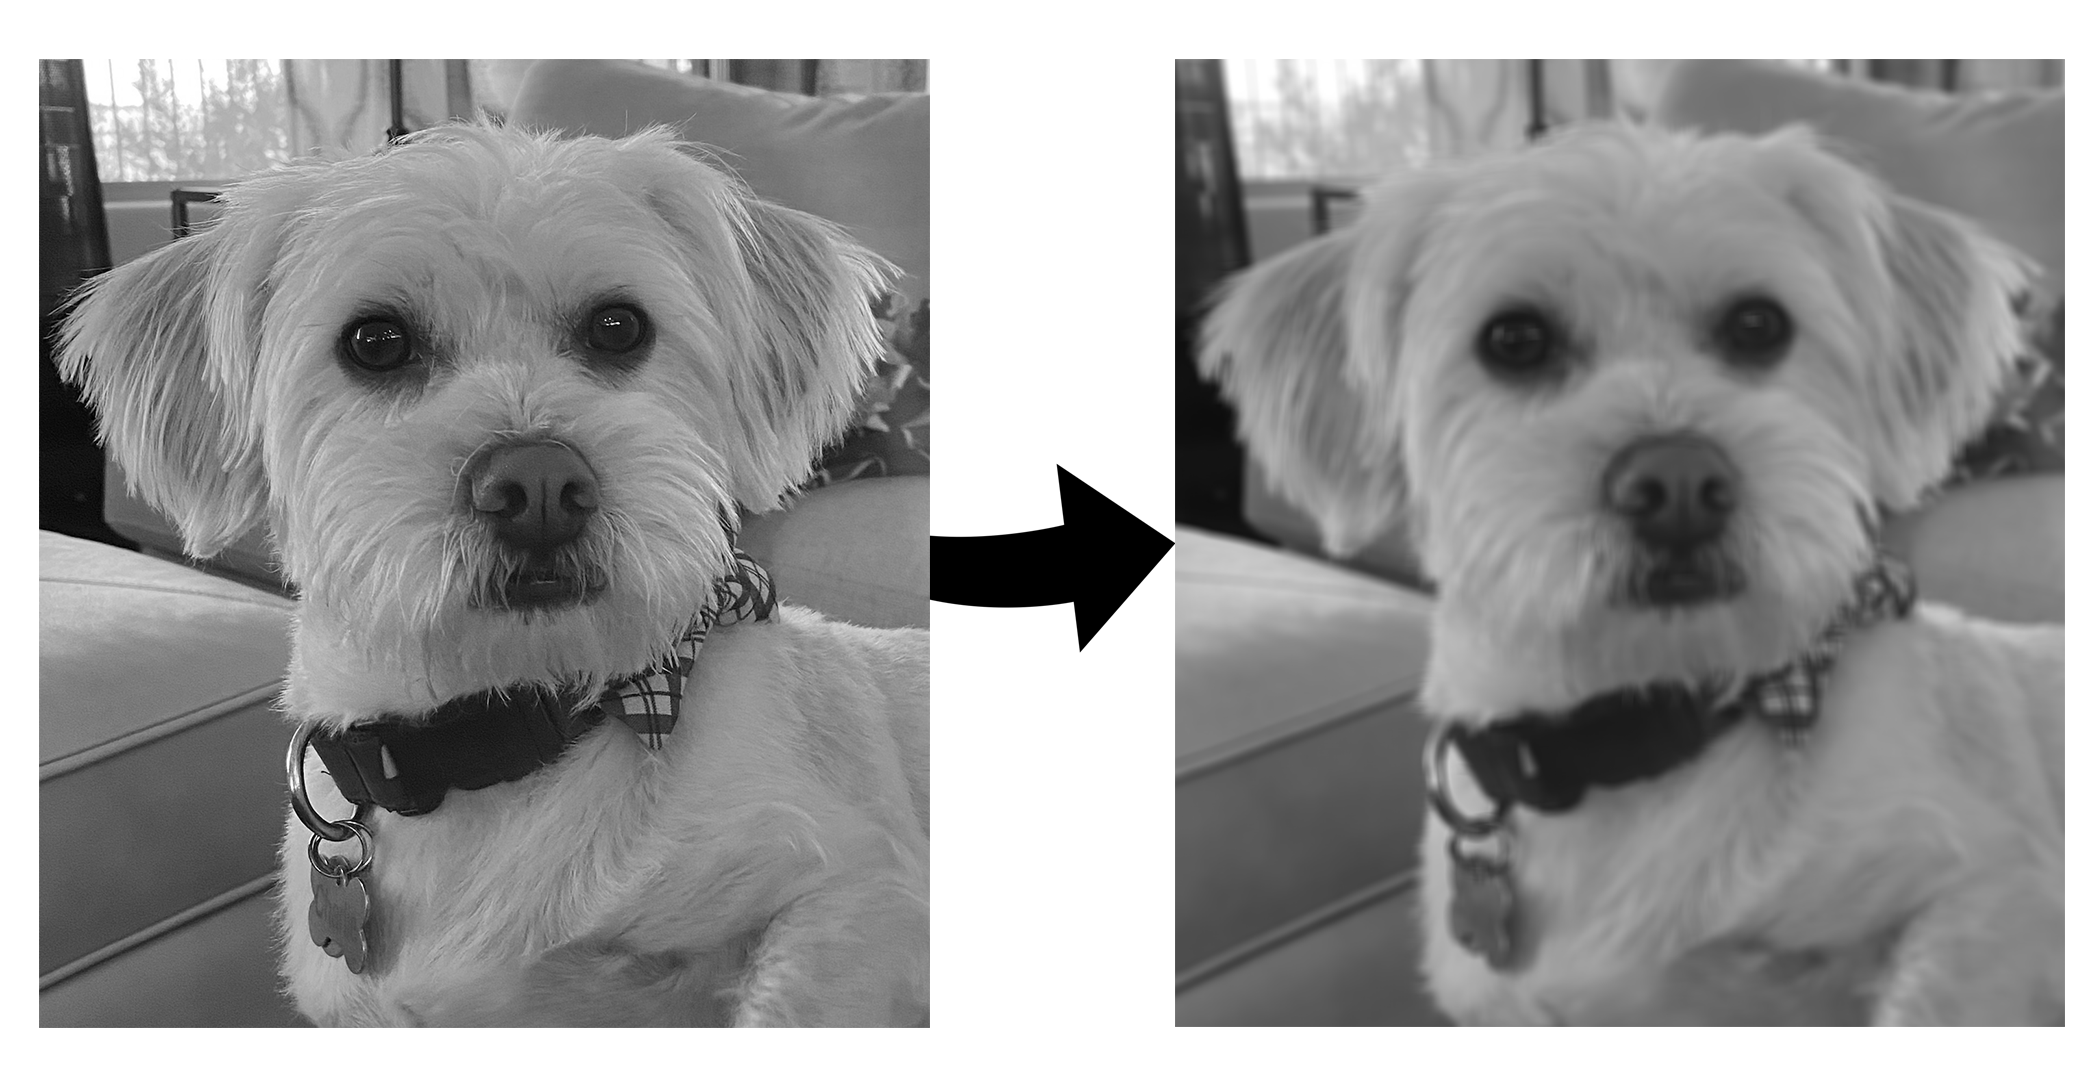
\includegraphics[width=100mm]{figures/GaussianExample2.png}
\centering
\caption{The effects of a Gaussian Blur.}
\label{augmentExample}
\end{figure}

\quad Both Millipyde and scikit-image's gaussian functions use two passes of a 1-dimensional Gaussian kernel which makes it a great example for comparison \cite{scipyGaussianSrc}. Millipyde also exploits the shared memory system on the GPU for the Gaussian function. A block of the input image is first loaded into shared memory so that each thread block has access to these pixel values. This technique was previously studied in CUDA, and it was shown to produce excellent results for GPU runtime \cite{cudaConvolution}. For this test, we used a sigma value of 2 for both Millipyde and scikit-image's benchmarks. To match the way Millipyde handle's pixel edge values and kernel widths, the following parameters were used for the scikit-image comparison:
\verb|cval=0|, \verb|truncate=8|, \verb|mode="constant"|. This ensures equal kernel sizes, and caps pixels outside of the image to a value of 0.


\begin{table}[H]
\centering
\begin{tabular}{ |c|c|c|c| } 
\hline
image size & scikit-image time (s) & Millipyde time (s) & \% difference \\
\hline
500&0.0105292&0.0002608&4037 \\
1000&0.0408449&0.0004123&9907 \\
1500&0.0902537&0.0006834&13207 \\
2000&0.1697805&0.0010704&15861 \\
2500&0.2523343&0.0015845&15925 \\
3000&0.3749286&0.0022314&16802 \\
3500&0.5563606&0.0029901&18607 \\
4000&0.7121980&0.0037107&19193 \\
4500&0.8735706&0.0047103&18546 \\
5000&1.0703184&0.0058559&18278 \\
5500&1.2964685&0.0069618&18623 \\
6000&1.5977196&0.0082425&19384 \\
\hline
\end{tabular}
\caption{Timing results for Gaussian blur using scikit-image and Millipyde.}
\label{gaussianTable}
\end{table}

\begin{figure}[H]
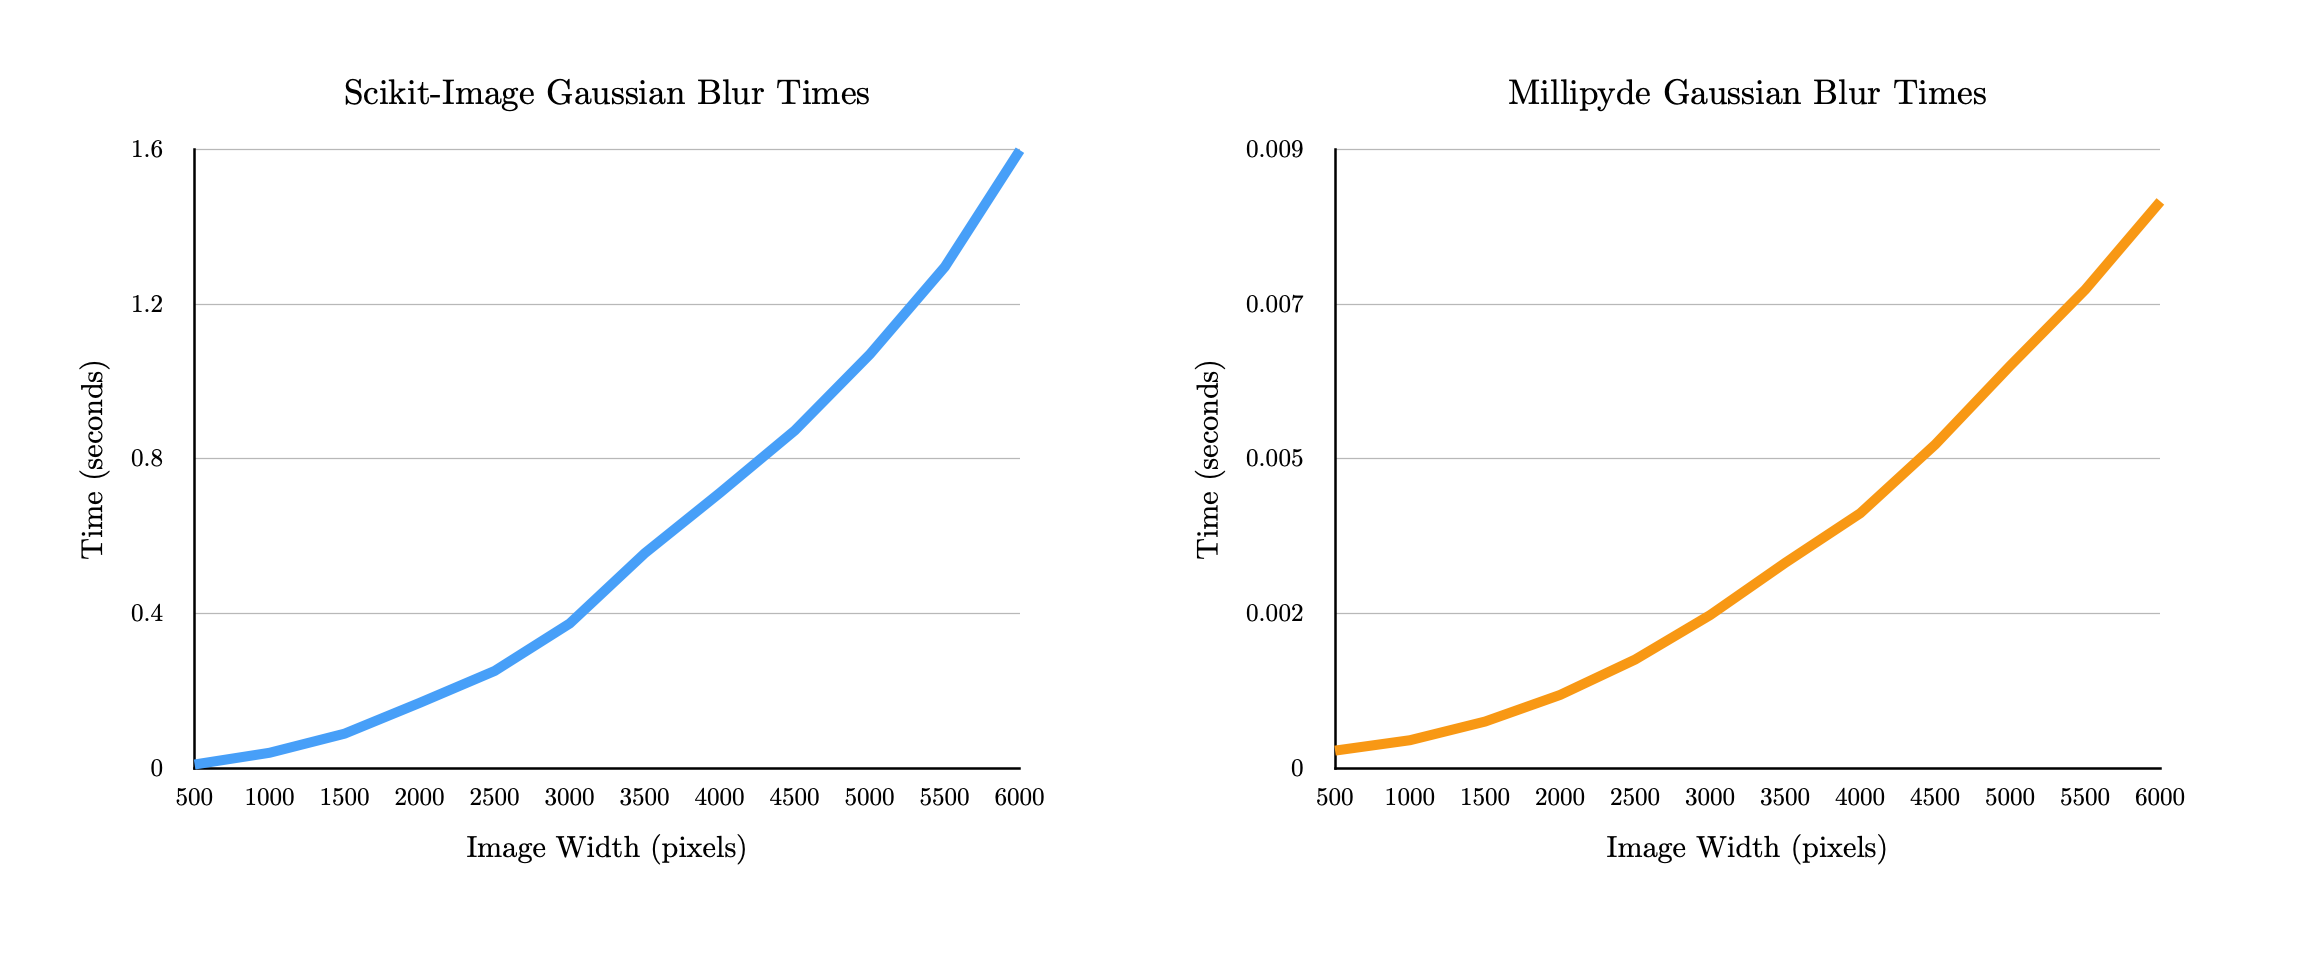
\includegraphics[width=\textwidth]{figures/gaussianComparison.png}
\centering
\caption{Graphical representation of the time spent performing a Gaussian blur on an image in scikit-image compared to its GPU-accelerated equivalent in Millipyde.}
\label{gaussianComparison}
\end{figure}

\quad This algorithm proved to be incredibly efficient in our Millipyde environment. As shown in Table \ref{gaussianTable} and Figure \ref{gaussianComparison}, our performance ranged from around 40x faster for smaller images up to just under 200x faster in larger images. Much of this performance increase is thanks to the shared memory blocks whose access times were much faster than always reading from global memory. This shows a lot of promise for future convolutional functions in Millipyde, and more experimentation should be done on utilizing shared memory in other image algorithms. 

\section{Pipeline Benchmarks}

Since our Pipeline objects exploit multiple forms of parallelism, it is worth studying the performance of various Pipeline configurations. Four our tests, we bench-marked the Pipelines using multiple copies of the same image for our list of inputs. Each image was 3500 pixels wide by 4666 pixels tall. The input list sizes ranged from 1 to 100. From there, four different configurations were run on each group of inputs. The first configuration, labeled `Control' in each respective chart, executed every Operation sequentially in a Python loop rather than using a Pipeline object at all. The test labeled `Single GPU' ran a single Pipeline that was bound to one given device so that it would not use all GPUs available on the system. The 3rd test, labeled `Dual GPUs' was not bound to a single device, so it was allowed to use both available devices for scheduling. The final test, labeled `Connected GPUs' split the work in half so that each of two Pipeline objects had half of the Operations to be completed. These two Pipelines were each bound to separate devices in the system and connected so that the outputs that completed on the first Pipeline would be transferred over to the second Pipeline to complete the remainder of the Operations.

\subsection{Pipelines with 5 Operations}

Our first experiment represented a standard small set of operations that may occur in a variety of data manipulation programs. Each iteration of the experiment used a total of five image transformation Operations. These included a Gaussian blur, gamma adjustment, horizontal flip, 45-degree rotation, and a greyscale conversion. For the connected Pipeline, these Operations were split in half so that the Gaussian blur, gamma adjustment, and flip were performed inside of the first Pipeline, and the rotation and greyscale conversion were performed on the second Pipeline.

\begin{table}[H]
\centering
\begin{tabular}{ |c|c|c|c|c| } 
\hline
Number of inputs & Control & Single GPU & Dual GPUs & Connected GPUs \\
\hline
1&	0.0244971&	0.0269347&	0.2622321&	0.0357248 \\
5&	0.1214234&	0.1228287&	0.1046105&	0.1197764\\
10&	0.2419561&	0.2456722&	0.1764512&	0.2654271\\
20&	0.4817377&	0.4817598&	0.3661450&	0.4735247\\
50&	1.2170164&	1.3320313&	0.8369642&	1.1232160\\
75&	1.9473421&	2.1429327&	1.2548219&	1.8599911\\
100&	2.9957998&	2.9042716&	1.6321600&	2.5250520\\
\hline
\end{tabular}
\caption{Timing results for running a short 5-Operation pipeline}
\label{pipelineTable1}
\end{table}

\begin{figure}[H]
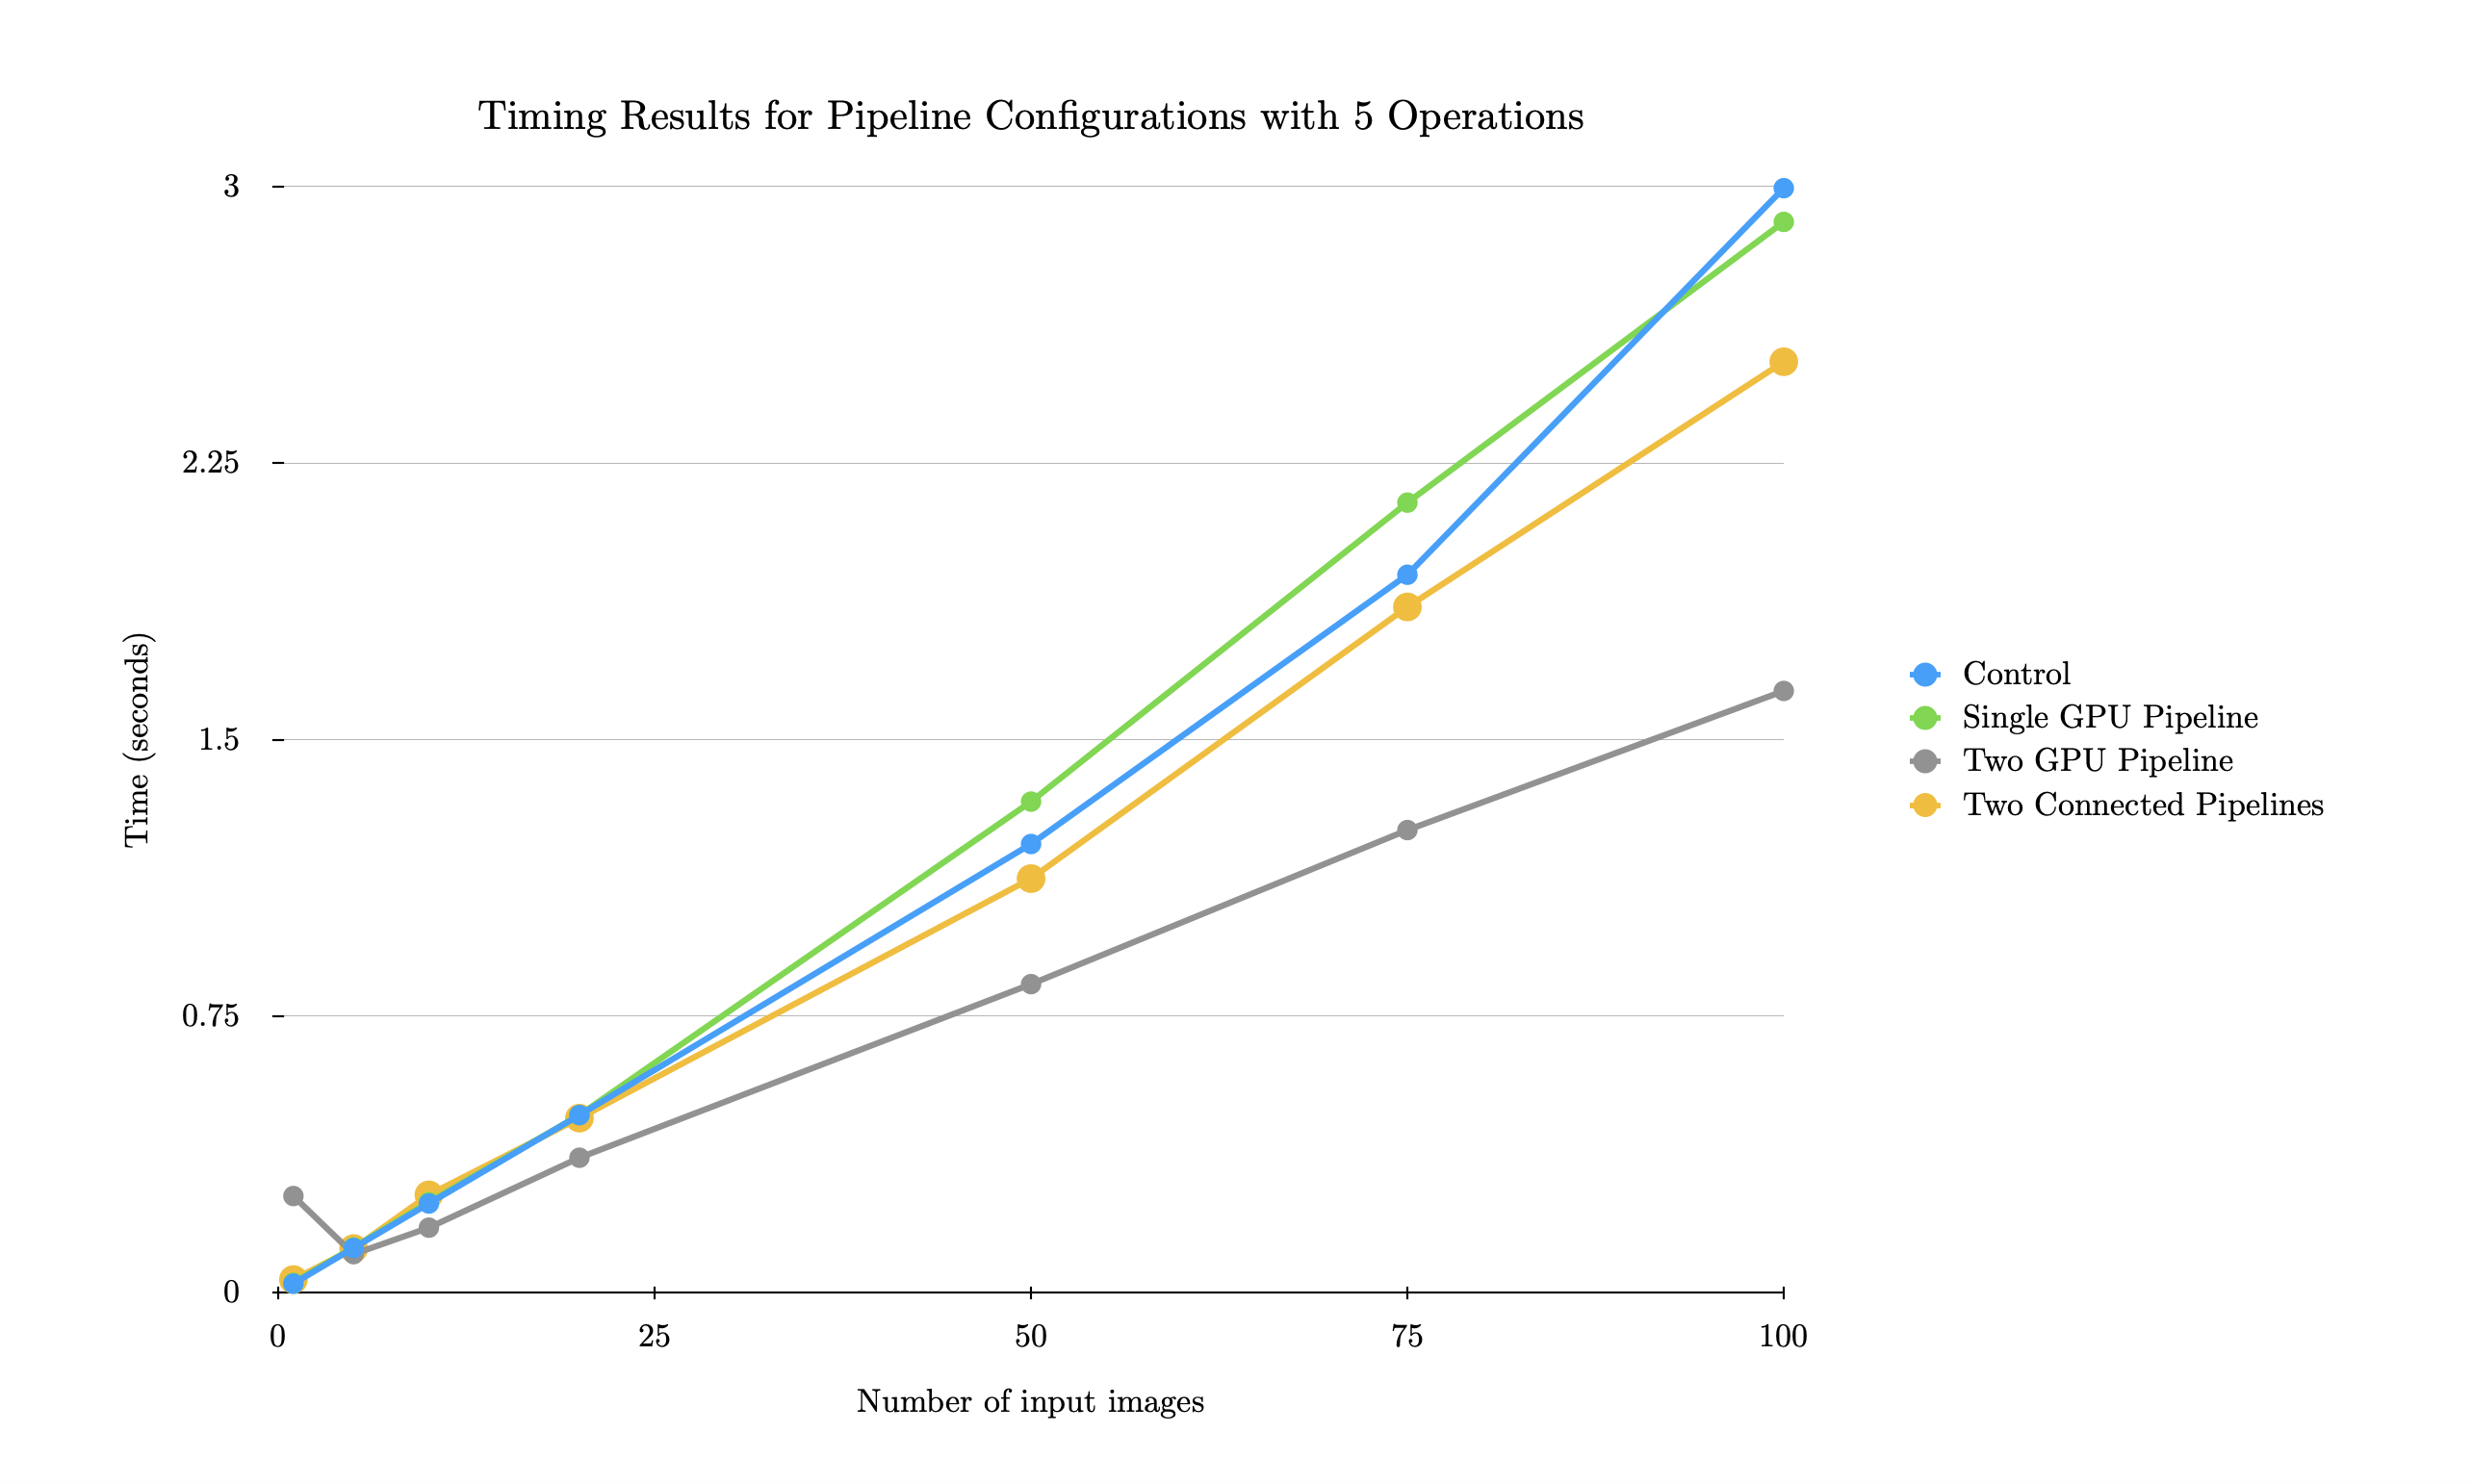
\includegraphics[width=\textwidth]{figures/pipelineChart1.png}
\centering
\caption{Graphical results for running a short 5-Operation pipeline.}
\label{pipelineChart1}
\end{figure}

\quad The results of this experiment are shown in Table \ref{pipelineTable1} and Figure \ref{pipelineChart1}. Predictably, the Pipeline that was able to use two GPUs performed the best. Its runtime was often half of the single-GPU Pipeline and the control experiment. The two connected Pipelines performed notably worse than the standard Pipeline despite the fact that both Pipelines should theoretically be splitting work across two GPUs. This is easily explained by the overhead from the transfer itself. When data is transferred from one Pipeline to the next, it has to be offloaded from the first device's work pool into the second device's work pool, and many small costs are incurred from operating managing both Pipeline objects simultaneously. 

\quad The single GPU pipeline showed disappointing performance that was often comparable to the control. Since the operations used were image-based transformations, little to no work was done on the CPU besides for immediate GPU kernel launches. This means that the work pools associated with each device were not fully utilized, and often only added scheduling overhead to the experiment. More work can be done in the future to make Millipyde's Pipeline scheduling more adaptable in these situations.

\subsection{CPU-bound Pipelines with 5 Operations}

To expose the effects of having the work pools associated with each device, we ran the same Pipeline tests as the previous experiment with the addition of simulated CPU work. At the beginning of each of the five Operations, 0.002 seconds of sleep was performed on the CPU. This was meant to represent time that could be incurred with future functions that require CPU-based kernel preparation prior to the kernel launch itself. Ideally, these experiments will be re-run and analyzed in the future when a function like this is added to Millipyde. 

\begin{table}[H]
\centering
\begin{tabular}{ |c|c|c|c|c| } 
\hline
Number of inputs & Control & Single GPU & Dual GPUs & Connected GPUs \\
\hline
1&	0.0373815&	0.0361518&	0.0370423&	0.0470410 \\
5&	0.1813750&	0.1406366&	0.1128026&	0.1417612 \\
10&	0.3653580&	0.2656119&	0.1972203&	0.2660218 \\
20&	0.7243550&	0.5269443&	0.3712618&	0.5205974 \\
50&	1.9165390&	1.6008312&	0.9192495&	1.2318530 \\
75&	3.0087808&	2.4173886&	1.3291795&	1.8750082 \\
100&	4.4714676&	3.3045429&	1.7332253&	2.5254060 \\
\hline
\end{tabular}
\caption{Timing results for running a 5-Operation pipeline with simulated CPU-bound pre-processing work.}
\label{pipelineTable2}
\end{table}

\begin{figure}[H]
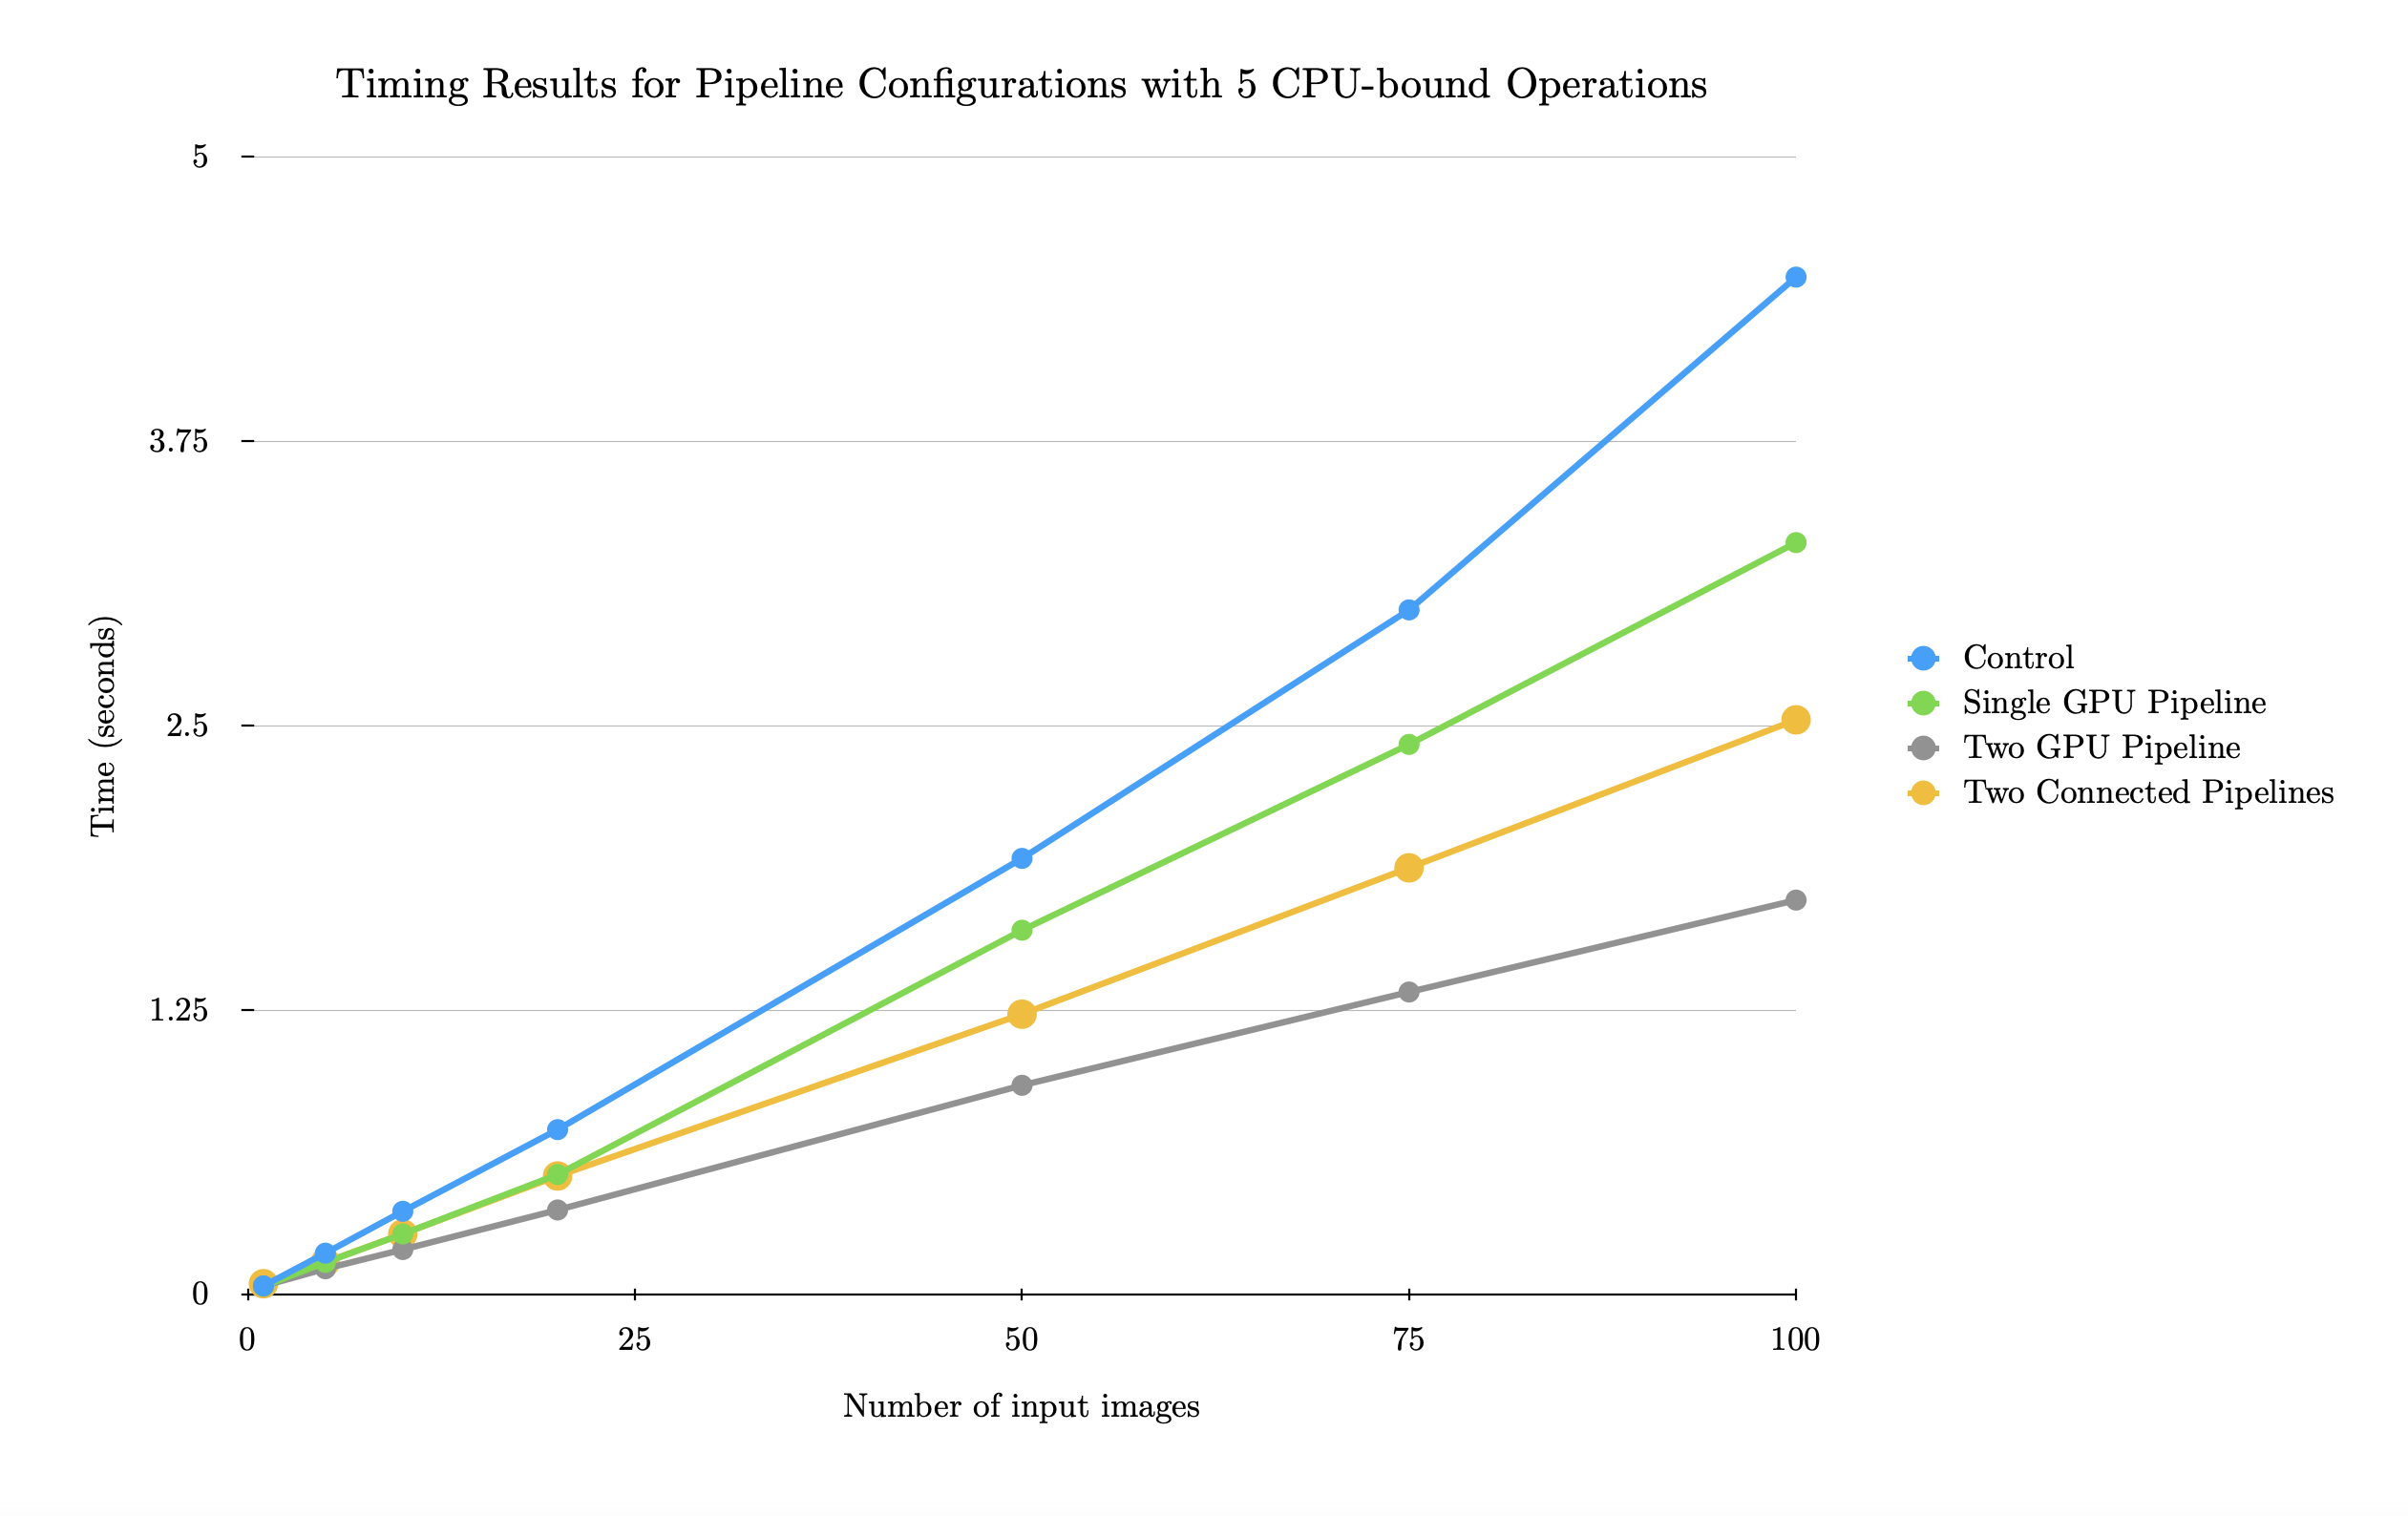
\includegraphics[width=\textwidth]{figures/pipelineChart3.png}
\centering
\caption{Timing results for running a 5-Operation pipeline with simulated CPU-bound pre-processing work.}
\label{pipelineChart2}
\end{figure}

As shown in Table \ref{pipelineTable2} and Figure \ref{pipelineChart2}, these results were more dramatic than the prior five-operation Pipeline experiment. The single-GPU pipeline was able to more predictably outperform the control experiment. We still saw strong performance gains from both of the two-GPU configurations. Despite this, the connected Pipelines still under-performed due to the cost of transferring the work from one Pipeline to the next.

\subsection{Pipelines with 20 Operations}

Lastly, an experiment was performed to see the effects of having longer Pipelines with many Operations. Each Pipeline in this test performed the same 20 Operations: seven Gaussian blurs, four gamma adjustments, two horizontal flips, six 45-degree rotations, and one greyscale conversion. This test is meant to represent more intensive GPU-operations that should further outweigh the costs incurred by the Pipeline's own overhead. For the two connected Pipelines, this work was split down the middle so that each Pipeline performed 10 Operations. 

\begin{table}[H]
\centering
\begin{tabular}{ |c|c|c|c|c| } 
\hline
Number of inputs & Control & Single GPU & Dual GPUs & Connected GPUs \\
\hline
1&	0.1210601&	0.1236825&	0.1229053&	0.1325121\\
5&	0.6136912&	0.6081436&	0.4897915&	0.5424913\\
10&	1.2329561&	1.2234442&	0.7826877&	0.8564503\\
20&	3.2071803&	2.9295116&	1.6075147&	1.6007919\\
50&	14.1225833&	17.9376053&	4.3081120&	4.4900887\\
75&	30.5186737&	30.8800205&	8.4228492&	8.4681248\\
100&	48.8984402&	46.5367387&	14.6403225&	14.5740577\\
\hline
\end{tabular}
\caption{Timing results for running a long 20-Operation Pipeline.}
\label{pipelineTable3}
\end{table}

\begin{figure}[H]
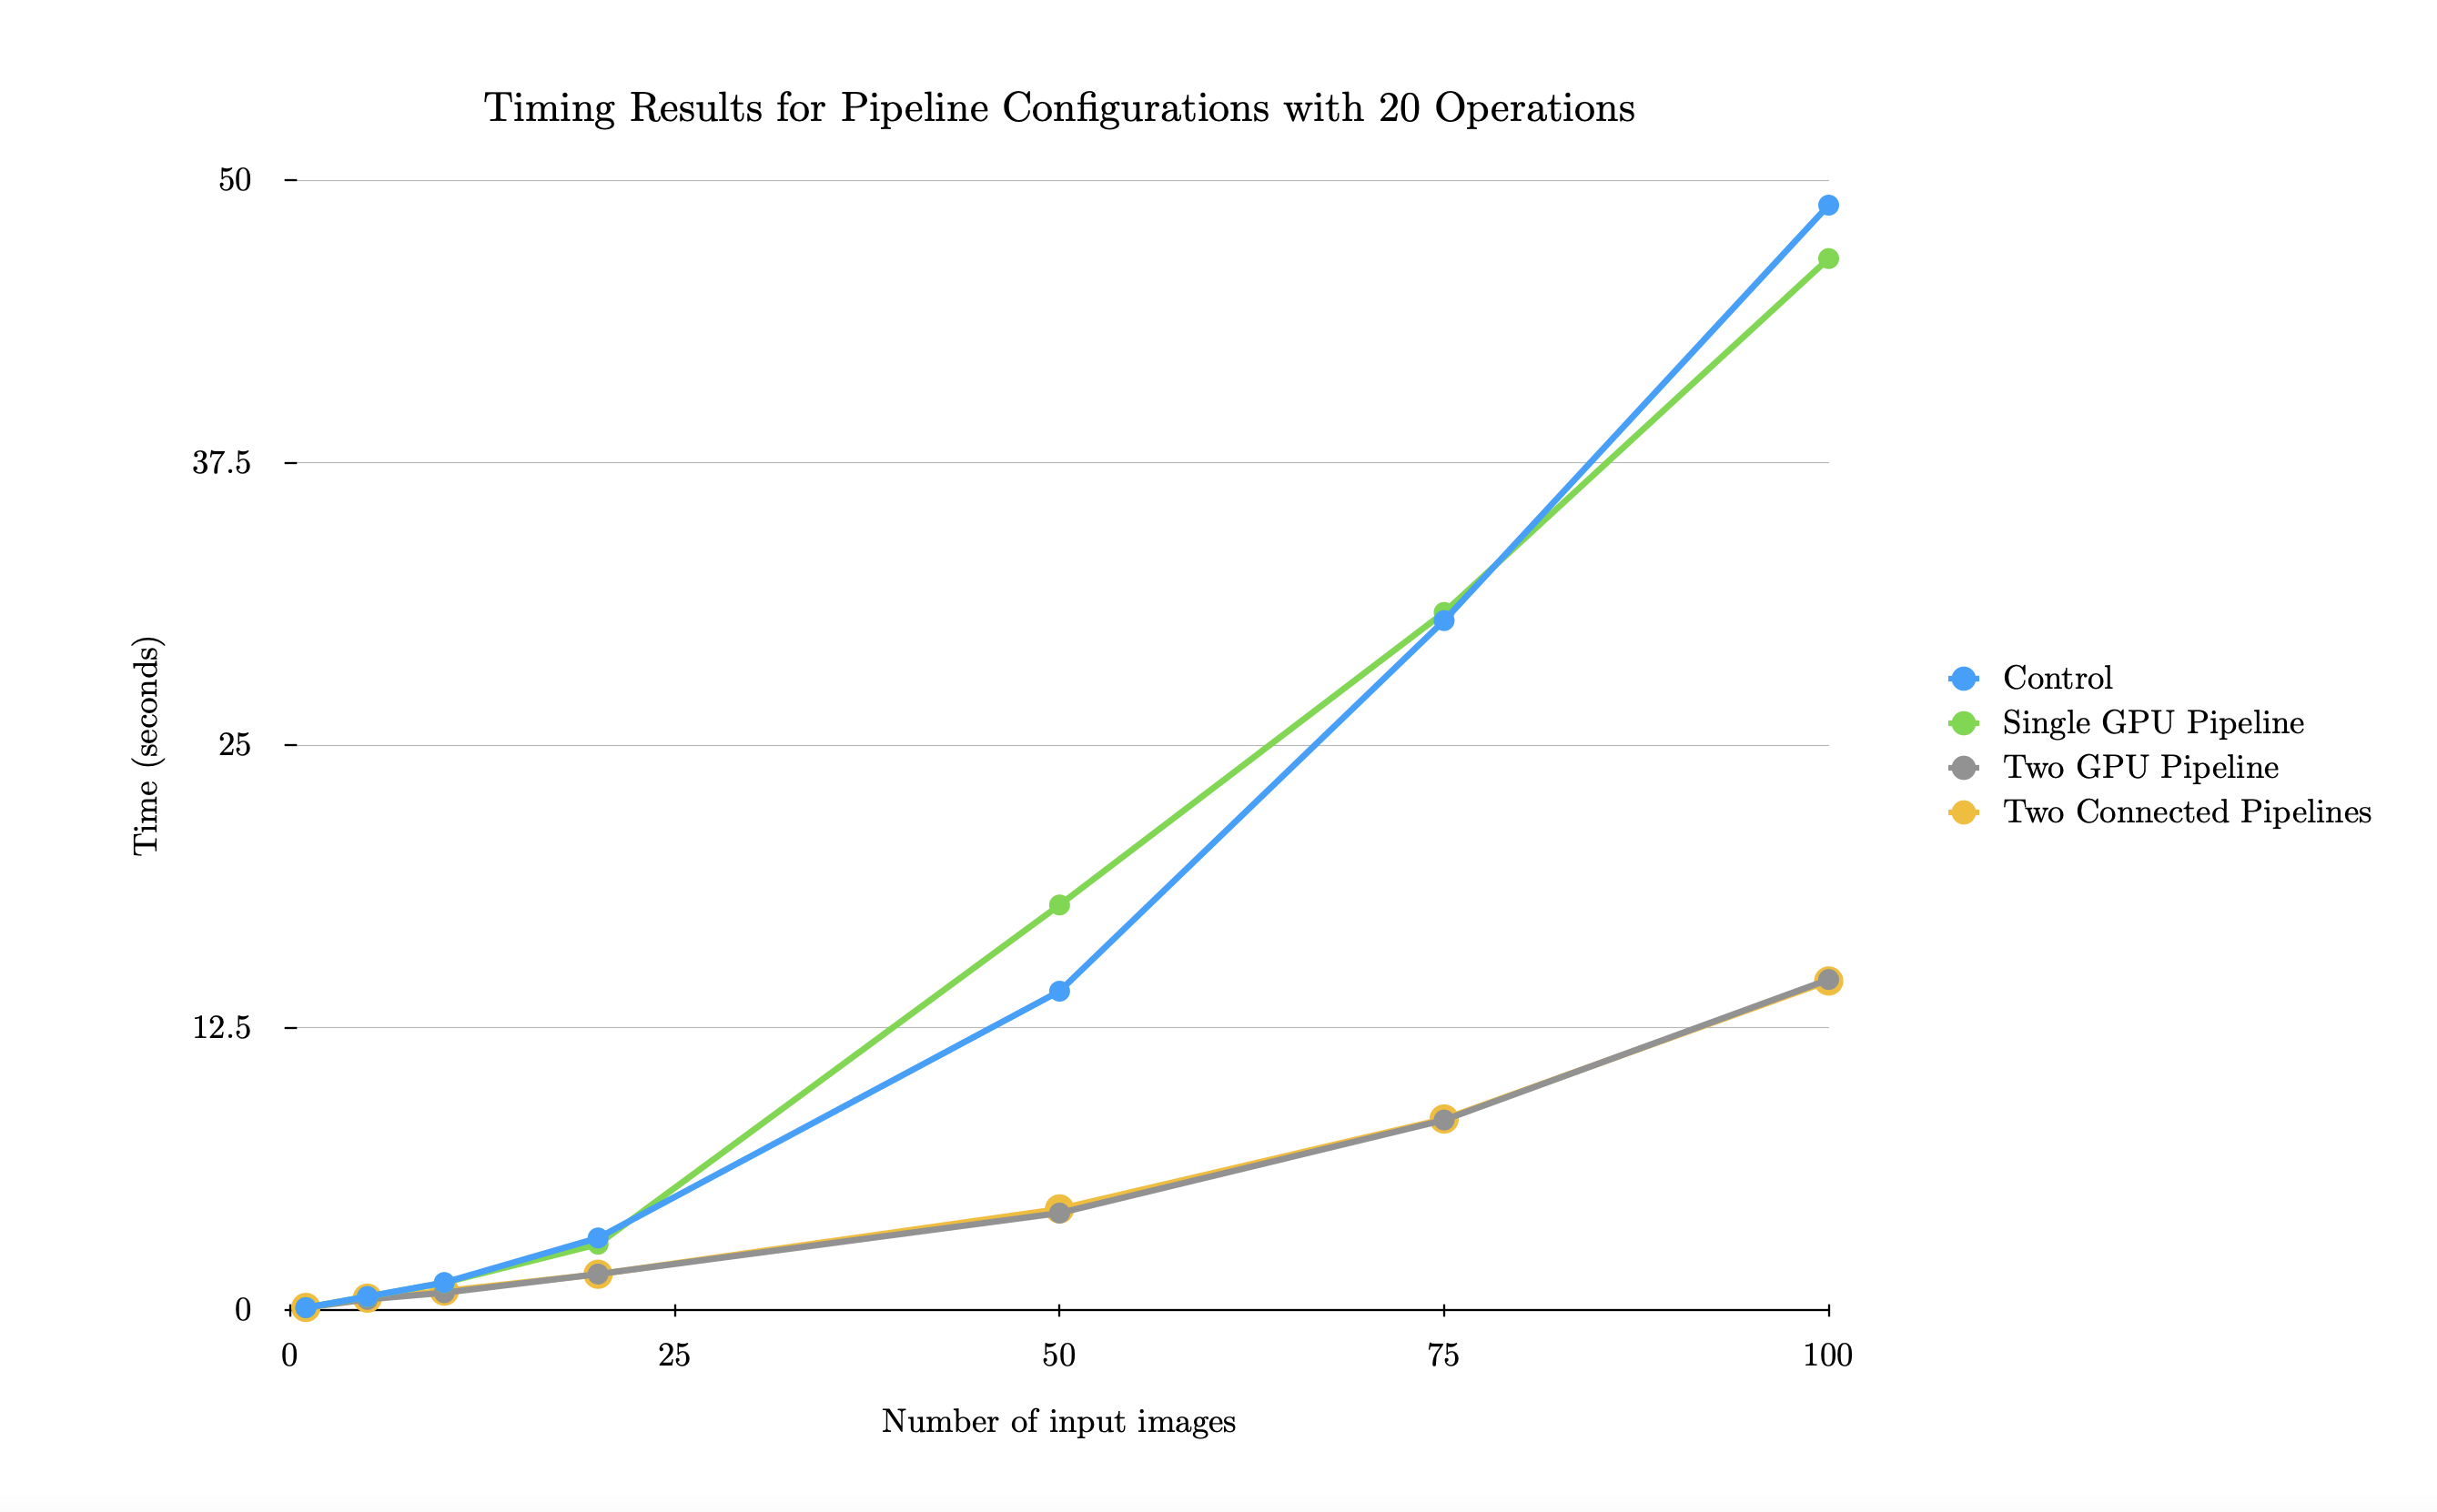
\includegraphics[width=\textwidth]{figures/pipelineChart2.png}
\centering
\caption{Graphical results for running a long 20-Operation Pipeline.}
\label{pipelineChart3}
\end{figure}

\quad As seen in Table \ref{pipelineTable3} and Figure \ref{pipelineChart3}, this experiment produced the most dramatic results. Now that the costs of Pipeline transfer were outweighed by the costs of the GPU computations, both dual-GPU configurations were able to perform roughly the same -- almost always within 0.1 seconds of each other. Surprisingly, both the control and the single-GPU pipeline performed poorly with more than double the runtime of their dual-GPU equivalents. 
